%%%%%%%%%%%%%%%%%%%%%%%%%%%%%%%%%%%%%%%%%%%%%%%%%%%%%%%%%%%%%%%%%%%%%%%%
%                                                                      %
%     File: Thesis_Introduction.tex                                    %
%     Tex Master: Thesis.tex                                           %
%                                                                      %
%     Author: Andre C. Marta                                           %
%     Last modified :  2 Jul 2015                                      %
%                                                                      %
%%%%%%%%%%%%%%%%%%%%%%%%%%%%%%%%%%%%%%%%%%%%%%%%%%%%%%%%%%%%%%%%%%%%%%%%

\chapter{Introduction}
\label{chapter:introduction}

With the advent of Big Data, a massive amount of information is continuously being collected and analyzed to extract meaning out of it. The way to obtain the value is through the use of machine learning (ML) algorithms, capable of analyzing massive data sets and uncover hidden relationships between the inputs, extracting meaning out of the raw information. From the panoply of ML algorithms, the category of Deep Learning (DL) is showing significant improvements in the capabilities of these models. 

The necessity of running DL algorithms in all kinds of devices, from supercomputers to smartphones, is appealing companies and researchers to the need to explore new ways of making these algorithms run faster while consuming less power. The tonic has been the exploration of Heterogeneous Computing Systems (HCS), composed of traditional Central Processing Units (CPUs) and Graphical Processing Units (GPUs). The use of GPUs, with their highly parallel architecture, is bringing significant gains in the performance of the processing systems and allowing for increased capabilities of the algorithms being run. 

The addition of this new processing device to the computers also brought the drawback added power consumption. However, unlike CPUs, where it is already common to see advance power techniques which control the frequency and voltage applied to the processor accordingly to the workload, on GPUs, the dynamic scaling of its frequency and voltage (dynamic voltage and frequency scaling - DVFS) is still mostly relying on external factors such as percentage of utilization, temperature of the die and power consumption. Nevertheless, even though GPUs are used in a vast type of applications (from video games and rendering, to scientific simulations and more recent deep learning applications), this is not preventing manufacturers from trying to optimize this device to coup with such different tasks. In the case of DL algorithms, significant efforts are being made to increase the efficiency of the GPUs running them. From optimizing specific parts of the GPU architecture to achieve higher performance, to smart computations scheduling, such that, the Dark Silicon phenomenon is minimized \cite{esmaeilzadeh_dark_2011}, to newer DVFS mechanisms that are aware to the running task type. 

If one looks to the nature of DL algorithms, the train of it is based on iterative and convergence processes, where small imprecisions on the computation, still lead to correct outputs. These types of applications can be classified as Imprecise Tolerant (IT) applications, and their hidden property of tolerance against imprecision can be exploited to increase the efficiency of the devices running them. In this case, two types of approaches can be made. First, the creation of custom computational blocks that natively hold sources of control imprecision intending to reduce the power consumption \cite{mahdiani_efficient_2017} or, second, try to use regular GPUs outside of the circumscribed voltage and frequency margins defined by the GPU manufacturer. While the first approach will require the addition of more hardware to the devices and contribute to the Dark Silicon phenomenon, the second has the increased benefit of allowing improvements to current hardware in the market. This advantage is of such significant importance, that conducted this dissertation automatically for this objective.

To verify the feasibility of enabling a degree of imprecise computation in a regular GPU, a convolution neural network (a type of deep learning algorithm specialized for image processing) is trained to identify handwritten numbers of the MNIST data set \cite{noauthor_mnist_1999}. This neural network is trained on a heterogeneous computer equipped with an AMD GPU, first with the conventional DVFS parameters and then with DVFS parameters outside of the conventional limits. It is verified that it is possible to undervolt the GPU core by 170mV without any degradation on both the performance of the GPU (required time to train the model) and the achieved accuracy at the end of the training session. More importantly, this reduction on the supplied voltage led to a reduction of 40.48\% of the maximum required power, a 28.81\% reduction on the average power, and a 26.92\% reduction of the total required energy spent to train the model.

This result shows that there is space to be explored outside of the conventional DVFS parameters when Imprecise Tolerant applications are being executed.


%%%%%%%%%%%%%%%%%%%%%%%%%%%%%%%%%%%%%%%%%%%%%%%%%%%%%%%%%%%%%%%%%%%%%%%%
\section{Main Objectives}
\label{section:objectives}

The objective of this dissertation is to create a novel DVFS mechanism aware of the nature of the application being run and the results produced by it. The new mechanism is applied to Deep Learning applications with the intention of reducing the power consumption of the GPU while maintaining the pic performance of the device. With this new mechanism, it will be possible to enlarge the voltage and frequency margins, working outside of the conventional DVFS limits in current hardware. 


The aspiration and contributions of this thesis can be decomposed on the following points:
\begin{itemize}
\item Acquire insight into the types of Deep Learning algorithms and their tolerance to imprecision.
\item Characterize the performance and power consumption of modern GPU architectures, working outside of conventional DVFS limits, first at a benchmark level and then concerning a variety of Deep Learning models.
\item Analyze and create a novel DVFS aware mechanism, able to extract meaningful power and performance gains on current GPU architectures.
\item Investigate the possibility and economic profits of the implementation of such a mechanism in large scale data centers.
\end{itemize}

Comparing the existing state of the art research against the presented dissertation, this work profits by performing not only the exploration of DVFS outside normal parameters but also by focusing on the impact of voltage scaling versus the traditional frequency scaling.  Figure \ref{fig:thesisObj} graphically shows the temporal relation between the different objectives to be performed during the dissertation.


\begin{figure}[!htb]
  \centering
  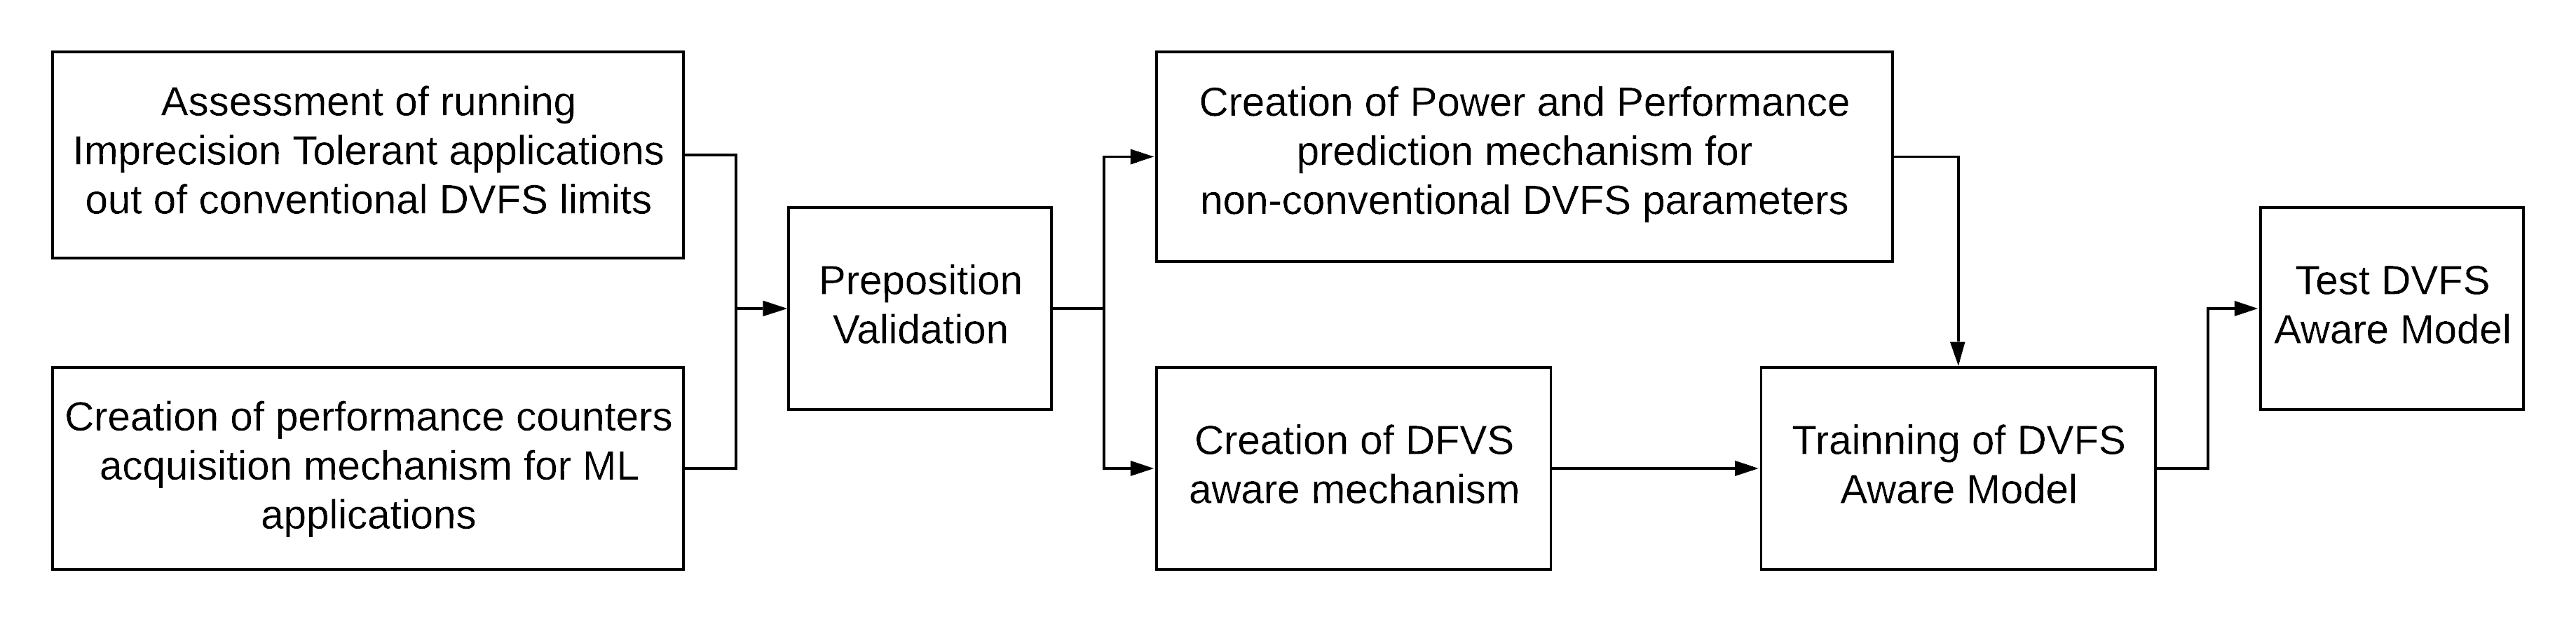
\includegraphics[width=1\textwidth]{Figures/Introduction/Dissertation_Objectives.png}
  \caption{Diagram of dissertation objectives.}
  \label{fig:thesisObj}
\end{figure}

\section{Report Outline}

In this report, a bibliographic review on the state of Graphical Processing Units architecture and current Dynamic Voltage and Frequency Scaling is performed; these include the foundations where the presented work is built on top. 

\begin{itemize}
\item In Chapter 1, an introduction and motivation over the impact of the research are presented.
\item In Chapter 2, a review of the background on GPU architecture, DVFS characterization and exploration, and current power and performance modeling techniques.
\item In Chapter 3, an overview of the target application that the novel DVFS mechanism exploration wants to focus on is given, and preliminary assessment results are shown.
\item In Chapter 4, an explanation of the work that is intended to be performed and developed during the dissertation is granted.

\end{itemize}